% Practice Test 25 — Virginia Edition
% Questions: 30 (21 MC + 9 SA)
% Generated by scripts/generate_practice_tests.py

\begin{practiceQuestion}{1-4-q26}{gmc}
\begin{questionText}
The graph below shows the cost of buying pounds of apples. Which equation matches this graph?

\begin{center}
\begin{tikzpicture}[scale=0.7]
  \draw[step=1,gray!20,thin] (0,0) grid (6,8);
  \draw[thick,->] (0,0) -- (6.5,0) node[right]{\small Pounds};
  \draw[thick,->] (0,0) -- (0,8.5) node[above]{\small Cost (\$)};
  \foreach \x in {1,...,6} \draw (\x,0.07) -- (\x,-0.07) node[below]{\tiny \x};
  \foreach \y in {1,...,8} \draw (0.07,\y) -- (-0.07,\y) node[left]{\tiny \y};
  \draw[thick,funBlue] (0,0) -- (6,7.5);
  \fill[funBlue] (0,0) circle (2.5pt);
  \fill[funBlue] (4,5) circle (2.5pt) node[above left]{\small $(4, 5)$};
\end{tikzpicture}
\end{center}
\end{questionText}
\choiceA{$c = 4p$}
\choiceB{$c = 1.25p$}
\choiceC{$c = 5p$}
\choiceD{$c = 0.8p$}
\correctAnswer{B}
\explanation{From the point $(4, 5)$: $k = \frac{5}{4} = 1.25$. The equation is $c = 1.25p$.}
\end{practiceQuestion}

\begin{practiceQuestion}{2-1-q26}{gmc}
\begin{questionText}
The $10 \times 10$ grid below has some squares shaded. What percent of the grid is shaded?

\begin{center}
\begin{tikzpicture}[scale=0.35]
  \foreach \x in {0,...,9} {
    \foreach \y in {0,...,9} {
      \draw[gray!50] (\x,\y) rectangle (\x+1,\y+1);
    }
  }
  % Shade 35 squares (rows 0-2 full = 30, plus 5 in row 3)
  \foreach \x in {0,...,9} {
    \foreach \y in {0,...,2} {
      \fill[funBlue!40] (\x,\y) rectangle (\x+1,\y+1);
      \draw[gray!50] (\x,\y) rectangle (\x+1,\y+1);
    }
  }
  \foreach \x in {0,...,4} {
    \fill[funBlue!40] (\x,3) rectangle (\x+1,4);
    \draw[gray!50] (\x,3) rectangle (\x+1,4);
  }
\end{tikzpicture}
\end{center}
\end{questionText}
\choiceA{$25\%$}
\choiceB{$30\%$}
\choiceC{$35\%$}
\choiceD{$40\%$}
\correctAnswer{C}
\explanation{The grid has $100$ squares total. Count the shaded squares: $3$ full rows of $10 = 30$, plus $5$ more $= 35$. So $35\%$ is shaded.}
\end{practiceQuestion}

\begin{practiceQuestion}{2-2-q02}{mc}
\begin{questionText}
Use a proportion to find $35\%$ of $120$.
\end{questionText}
\choiceA{$35$}
\choiceB{$38$}
\choiceC{$42$}
\choiceD{$48$}
\correctAnswer{C}
\explanation{Set up $\frac{n}{120} = \frac{35}{100}$. Cross-multiply: $100n = 4200$. Divide: $n = 42$.}
\end{practiceQuestion}

\begin{practiceQuestion}{2-3-q15}{mc}
\begin{questionText}
Which of the following results in the greatest final value, starting from $\$100$?
\end{questionText}
\choiceA{Increase by $30\%$}
\choiceB{Increase by $20\%$, then increase by $10\%$}
\choiceC{Increase by $15\%$ twice}
\choiceD{All give the same result}
\correctAnswer{C}
\explanation{A: $100 \times 1.30 = 130$. B: $100 \times 1.20 \times 1.10 = 132$. C: $100 \times 1.15 \times 1.15 = 132.25$. C is the greatest.}
\end{practiceQuestion}

\begin{practiceQuestion}{2-7-q18}{mc}
\begin{questionText}
A package was estimated to weigh $10$ kg, but it actually weighs $12$ kg. A second package was estimated to weigh $50$ kg, but it actually weighs $52$ kg. Which estimate has the smaller percent error?
\end{questionText}
\choiceA{The first package}
\choiceB{The second package}
\choiceC{They have the same percent error}
\choiceD{Cannot be determined}
\correctAnswer{B}
\explanation{First: $\frac{2}{12} \times 100 \approx 16.7\%$. Second: $\frac{2}{52} \times 100 \approx 3.8\%$. The second has a smaller percent error.}
\end{practiceQuestion}

\begin{practiceQuestion}{3-2-q30}{gsa}
\begin{questionText}
A thermometer shows temperature changes over three hours.

\begin{center}
\begin{tikzpicture}
  \draw[thick,->] (0,-4.5) -- (0,4.5);
  \foreach \y in {-4,...,4} \draw (-0.15,\y) -- (0.15,\y) node[right=4pt] {$\y°$C};
  \fill[funBlue] (0,-3) circle (4pt);
  \node[left=8pt] at (0,-3) {Start: $-3°$C};
  \draw[thick,->,funGreen] (-0.6,-3) -- (-0.6,1);
  \node[left] at (-0.6,-1) {\footnotesize $+4°$};
  \draw[thick,->,funRed] (-1.2,1) -- (-1.2,-2);
  \node[left] at (-1.2,-0.5) {\footnotesize $-3°$};
\end{tikzpicture}
\end{center}

What is the final temperature after these two changes?
\end{questionText}
\correctAnswer{$-2°$C}
\explanation{Start at $-3°$C. Rise $4°$: $-3 + 4 = 1°$C. Drop $3°$: $1 + (-3) = -2°$C.}
\end{practiceQuestion}

\begin{practiceQuestion}{3-3-q20}{sa}
\begin{questionText}
What is $(-8) - (-15)$?
\end{questionText}
\correctAnswer{$7$}
\explanation{$(-8) - (-15) = (-8) + 15 = 7$.}
\end{practiceQuestion}

\begin{practiceQuestion}{3-4-q22}{sa}
\begin{questionText}
A hiker descends from an elevation of $-15.4$ meters to $-23.8$ meters. How many meters did the hiker descend?
\end{questionText}
\correctAnswer{$8.4$ meters}
\explanation{Change: $-23.8 - (-15.4) = -23.8 + 15.4 = -8.4$. The hiker descended $8.4$ meters.}
\end{practiceQuestion}

\begin{practiceQuestion}{4-3-q04}{mc}
\begin{questionText}
Expand $-4(2y - 5)$.
\end{questionText}
\choiceA{$-8y - 20$}
\choiceB{$-8y - 5$}
\choiceC{$-8y + 20$}
\choiceD{$8y + 20$}
\correctAnswer{C}
\explanation{$-4 \times 2y = -8y$ and $-4 \times (-5) = +20$. A negative times a negative is positive. Result: $-8y + 20$.}
\end{practiceQuestion}

\begin{practiceQuestion}{4-4-q04}{mc}
\begin{questionText}
Which is the completely factored form of $8m + 20$?
\end{questionText}
\choiceA{$2(4m + 10)$}
\choiceB{$4(2m + 5)$}
\choiceC{$8(m + 20)$}
\choiceD{$4(2m + 20)$}
\correctAnswer{B}
\explanation{GCF of $8$ and $20$ is $4$. Factor: $8m \div 4 = 2m$ and $20 \div 4 = 5$. Result: $4(2m + 5)$. Choice A uses $2$, which is not the GCF.}
\end{practiceQuestion}

\begin{practiceQuestion}{5-4-q29}{gsa}
\begin{questionText}
The bar graph shows how much three students earned. Together they earned a total of $\$31.50$. Student C earned $\dfrac{1}{2}$ as much as Student A. Find how much Student C earned.

\begin{center}
\begin{tikzpicture}[scale=0.5]
  \draw[thick,->] (0,0) -- (0,11) node[above] {Dollars (\$)};
  \draw[thick,->] (0,0) -- (10,0);
  % Bars
  \draw[thick,fill=funBlue!40] (1,0) rectangle (3,8);
  \node[below] at (2,-0.3) {A};
  \node at (2,8.5) {$\$12$};
  \draw[thick,fill=funOrange!40] (4,0) rectangle (6,0);
  \node[below] at (5,-0.3) {B};
  \node at (5,1) {?};
  \draw[thick,fill=funGreen!40] (7,0) rectangle (9,0);
  \node[below] at (8,-0.3) {C};
  \node at (8,1) {?};
  % Y-axis labels
  \foreach \y in {0,2,...,10} {
    \draw (-0.2,\y) -- (0,\y);
    \node[left] at (-0.3,\y) {$\y$};
  }
\end{tikzpicture}
\end{center}

Student A earned $\$12$, and Student C earned $\dfrac{1}{2}$ of Student A's earnings.
\end{questionText}
\correctAnswer{$\$6$}
\explanation{Student C $= \frac{1}{2} \times 12 = \$6$. Check: Student B $= 31.50 - 12 - 6 = \$13.50$. Total: $12 + 13.50 + 6 = 31.50$ \checkmark.}
\end{practiceQuestion}

\begin{practiceQuestion}{5-5-q14}{mc}
\begin{questionText}
Solve $7 - 2x < 1$.
\end{questionText}
\choiceA{$x < 3$}
\choiceB{$x > 3$}
\choiceC{$x < -3$}
\choiceD{$x > -3$}
\correctAnswer{B}
\explanation{Subtract $7$: $-2x < -6$. Divide by $-2$ and flip: $x > 3$.}
\end{practiceQuestion}

\begin{practiceQuestion}{5-6-q29}{gsa}
\begin{questionText}
Solve $-3x + 9 > 0$. Then graph the solution on the number line below by describing the circle type and shading direction.

\begin{center}
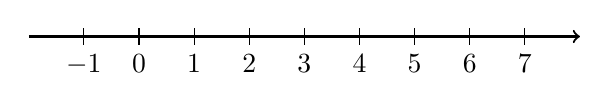
\begin{tikzpicture}[scale=0.7]
  \draw[thick,->] (-2,0) -- (8,0);
  \foreach \x in {-1,...,7} \draw (\x,0.15) -- (\x,-0.15) node[below] {$\x$};
\end{tikzpicture}
\end{center}
\end{questionText}
\correctAnswer{$x < 3$; open circle at $3$, shade left}
\explanation{Subtract $9$: $-3x > -9$. Divide by $-3$ and flip: $x < 3$. Open circle at $3$, shade left.}
\end{practiceQuestion}

\begin{practiceQuestion}{6-1-q18}{mc}
\begin{questionText}
A rectangular swimming pool is $6$ cm by $2.5$ cm on a drawing with scale $1$ cm $= 8$ m. What is the actual perimeter of the pool?
\end{questionText}
\choiceA{$17$ m}
\choiceB{$68$ m}
\choiceC{$136$ m}
\choiceD{$960$ m}
\correctAnswer{C}
\explanation{Actual dimensions: $6 \times 8 = 48$ m and $2.5 \times 8 = 20$ m. Perimeter: $2(48 + 20) = 2(68) = 136$ m.}
\end{practiceQuestion}

\begin{practiceQuestion}{6-2-q18}{mc}
\begin{questionText}
A drawing uses $1$ cm $= 5$ km. A road is $7$ cm long. Another map shows the same road as $3.5$ cm. What is the scale of the second map?
\end{questionText}
\choiceA{$1$ cm $= 2.5$ km}
\choiceB{$1$ cm $= 5$ km}
\choiceC{$1$ cm $= 10$ km}
\choiceD{$1$ cm $= 17.5$ km}
\correctAnswer{C}
\explanation{Actual road: $7 \times 5 = 35$ km. New scale: $35 \div 3.5 = 10$. So the second map uses $1$ cm $= 10$ km.}
\end{practiceQuestion}

\begin{practiceQuestion}{6-5-q19}{sa}
\begin{questionText}
What shape is the cross-section when you cut a sphere through its center?
\end{questionText}
\correctAnswer{A circle (the largest possible circle)}
\explanation{A cut through the center of a sphere produces a great circle — the largest possible circular cross-section, with the same radius as the sphere.}
\end{practiceQuestion}

\begin{practiceQuestion}{6-6-q13}{mc}
\begin{questionText}
Two lines intersect. One angle formed is $130°$. What are the measures of all four angles?
\end{questionText}
\choiceA{$130°$, $130°$, $50°$, $50°$}
\choiceB{$130°$, $50°$, $130°$, $100°$}
\choiceC{$130°$, $130°$, $130°$, $130°$}
\choiceD{$130°$, $60°$, $130°$, $40°$}
\correctAnswer{A}
\explanation{Vertical angles are equal ($130°$ and $130°$). Adjacent angles are supplementary: $180° - 130° = 50°$. The four angles are $130°$, $50°$, $130°$, $50°$.}
\end{practiceQuestion}

\begin{practiceQuestion}{6-7-q29}{gsa}
\begin{questionText}
The coordinate plane shows a rectangle with vertices $A(1, 1)$, $B(5, 1)$, $C(5, 3)$, $D(1, 3)$. Reflect the rectangle over the $x$-axis and list the new vertices.

\begin{center}
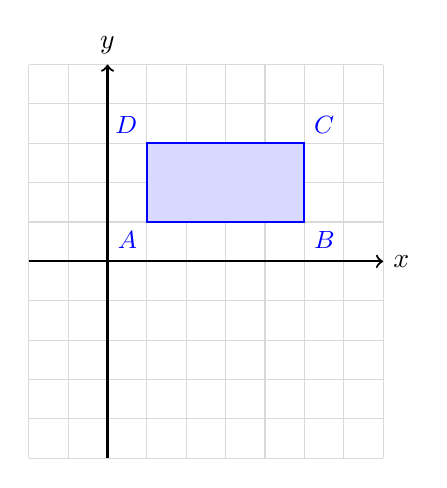
\begin{tikzpicture}[scale=0.5]
  \draw[step=1,gray!30,thin] (-2,-5) grid (7,5);
  \draw[thick,->] (-2,0) -- (7,0) node[right]{$x$};
  \draw[thick,->] (0,-5) -- (0,5) node[above]{$y$};
  \draw[thick,blue,fill=blue!15] (1,1) -- (5,1) -- (5,3) -- (1,3) -- cycle;
  \node[above left,blue,font=\small] at (1,3) {$D$};
  \node[above right,blue,font=\small] at (5,3) {$C$};
  \node[below left,blue,font=\small] at (1,1) {$A$};
  \node[below right,blue,font=\small] at (5,1) {$B$};
\end{tikzpicture}
\end{center}
\end{questionText}
\correctAnswer{$A'(1, -1)$, $B'(5, -1)$, $C'(5, -3)$, $D'(1, -3)$}
\explanation{Over the $x$-axis: keep $x$, negate $y$. $(1,1) \to (1,-1)$, $(5,1) \to (5,-1)$, $(5,3) \to (5,-3)$, $(1,3) \to (1,-3)$.}
\end{practiceQuestion}

\begin{practiceQuestion}{6-8-q10}{mc}
\begin{questionText}
A building is $60$ ft tall and casts a $40$-ft shadow. A nearby tree casts a $12$-ft shadow. How tall is the tree?
\end{questionText}
\choiceA{$8$ ft}
\choiceB{$12$ ft}
\choiceC{$18$ ft}
\choiceD{$20$ ft}
\correctAnswer{C}
\explanation{$\frac{60}{40} = \frac{h}{12}$. Cross-multiply: $40h = 720$. Divide: $h = 18$ ft.}
\end{practiceQuestion}

\begin{practiceQuestion}{7-4-q05}{mc}
\begin{questionText}
A rectangular yard is $20$ m by $15$ m. A circular flower bed with radius $3$ m is in the center. What is the area of the yard NOT covered by the flower bed? Use $\pi \approx 3.14$.
\end{questionText}
\choiceA{$271.74$ m$^2$}
\choiceB{$300$ m$^2$}
\choiceC{$328.26$ m$^2$}
\choiceD{$28.26$ m$^2$}
\correctAnswer{A}
\explanation{Yard: $20 \times 15 = 300$ m$^2$. Circle: $3.14 \times 9 = 28.26$ m$^2$. Remaining: $300 - 28.26 = 271.74$ m$^2$.}
\end{practiceQuestion}

\begin{practiceQuestion}{7-5-q01}{mc}
\begin{questionText}
What is the surface area of a cube with side length $4$ cm?
\end{questionText}
\choiceA{$16$ cm$^2$}
\choiceB{$64$ cm$^2$}
\choiceC{$96$ cm$^2$}
\choiceD{$24$ cm$^2$}
\correctAnswer{C}
\explanation{A cube has $6$ faces. $SA = 6s^2 = 6 \times 16 = 96$ cm$^2$.}
\end{practiceQuestion}

\begin{practiceQuestion}{7-6-q11}{mc}
\begin{questionText}
A triangular prism has a triangular base with legs $5$ cm and $12$ cm (right triangle). The prism is $15$ cm long. What is the volume?
\end{questionText}
\choiceA{$150$ cm$^3$}
\choiceB{$300$ cm$^3$}
\choiceC{$450$ cm$^3$}
\choiceD{$900$ cm$^3$}
\correctAnswer{C}
\explanation{$B = \frac{1}{2} \times 5 \times 12 = 30$ cm$^2$. $V = 30 \times 15 = 450$ cm$^3$.}
\end{practiceQuestion}

\begin{practiceQuestion}{7-7-q23}{sa}
\begin{questionText}
A cylindrical swimming pool has a radius of $5$ m and a depth of $2$ m. How many cubic meters of water does it hold? Use $\pi \approx 3.14$.
\end{questionText}
\correctAnswer{$157$ m$^3$}
\explanation{$V = \pi r^2 h = 3.14 \times 25 \times 2 = 157$ m$^3$.}
\end{practiceQuestion}

\begin{practiceQuestion}{8-1-q28}{gmc}
\begin{questionText}
The table below shows the results of two samples taken from a population of $1{,}000$ students.

\begin{center}
\begin{tabular}{|l|c|c|}
\hline
 & \textbf{Sample 1 (50 students)} & \textbf{Sample 2 (50 students)} \\
\hline
Prefer Math & $18$ & $22$ \\
\hline
Prefer Science & $14$ & $12$ \\
\hline
Prefer English & $10$ & $8$ \\
\hline
Prefer Art & $8$ & $8$ \\
\hline
\end{tabular}
\end{center}

Based on both samples, the best prediction for how many of the $1{,}000$ students prefer math is:
\end{questionText}
\choiceA{$180$}
\choiceB{$220$}
\choiceC{$400$}
\choiceD{$360$}
\correctAnswer{C}
\explanation{Average the two samples: $\frac{18+22}{2} = 20$ out of $50 = 40\%$. Then $40\%$ of $1{,}000 = 400$.}
\end{practiceQuestion}

\begin{practiceQuestion}{8-3-q16}{mc}
\begin{questionText}
Two histograms show that Group A's data is skewed left and Group B's data is symmetric. Which measure of center is most appropriate to compare them?
\end{questionText}
\choiceA{Mean for both}
\choiceB{Median for both}
\choiceC{Mode for both}
\choiceD{Range for both}
\correctAnswer{B}
\explanation{The median is less affected by skew than the mean, so it is the best measure to compare a skewed and a symmetric distribution.}
\end{practiceQuestion}

\begin{practiceQuestion}{8-4-q23}{sa}
\begin{questionText}
Data: $100, 200, 300, 400, 500$. Find the median and the IQR.
\end{questionText}
\correctAnswer{Median $= 300$; IQR $= 200$}
\explanation{Median (3rd value) $= 300$. $Q_1 = 200$, $Q_3 = 400$. IQR $= 400 - 200 = 200$.}
\end{practiceQuestion}

\begin{practiceQuestion}{8-5-q02}{mc}
\begin{questionText}
Which of the following is true about the leaves in a stem-and-leaf plot?
\end{questionText}
\choiceA{Leaves are listed in random order}
\choiceB{Leaves are listed in order from least to greatest}
\choiceC{Each leaf represents the tens digit}
\choiceD{Leaves are always single digits from $1$ to $9$}
\correctAnswer{B}
\explanation{Leaves must be arranged in order from least to greatest so the data is easy to read.}
\end{practiceQuestion}

\begin{practiceQuestion}{9-3-q26}{gmc}
\begin{questionText}
The bar graph shows the results of rolling a die $60$ times. Based on the graph, what is the experimental probability of rolling a $3$?

\begin{center}
\begin{tikzpicture}[scale=0.55]
  \draw[thick,->] (0,0) -- (0,14) node[above,font=\small] {Frequency};
  \draw[thick,->] (0,0) -- (8,0);
  \foreach \y in {2,4,...,12} {
    \draw[gray!30] (0,\y) -- (7.5,\y);
    \node[left,font=\small] at (0,\y) {\y};
  }
  \fill[funBlue!70] (0.3,0) rectangle (1,8);
  \fill[funBlue!70] (1.3,0) rectangle (2,12);
  \fill[funBlue!70] (2.3,0) rectangle (3,6);
  \fill[funBlue!70] (3.3,0) rectangle (4,10);
  \fill[funBlue!70] (4.3,0) rectangle (5,14);
  \fill[funBlue!70] (5.3,0) rectangle (6,10);
  \node[below,font=\small] at (0.65,0) {1};
  \node[below,font=\small] at (1.65,0) {2};
  \node[below,font=\small] at (2.65,0) {3};
  \node[below,font=\small] at (3.65,0) {4};
  \node[below,font=\small] at (4.65,0) {5};
  \node[below,font=\small] at (5.65,0) {6};
\end{tikzpicture}
\end{center}
\end{questionText}
\choiceA{$\frac{6}{60}$}
\choiceB{$\frac{10}{60}$}
\choiceC{$\frac{12}{60}$}
\choiceD{$\frac{14}{60}$}
\correctAnswer{A}
\explanation{The bar for $3$ reaches $6$. $P = \frac{6}{60} = \frac{1}{10}$.}
\end{practiceQuestion}

\begin{practiceQuestion}{9-6-q15}{mc}
\begin{questionText}
Two dice are rolled. What is the probability that the product (not the sum) of the two numbers is $12$?
\end{questionText}
\choiceA{$\frac{2}{36}$}
\choiceB{$\frac{4}{36}$}
\choiceC{$\frac{3}{36}$}
\choiceD{$\frac{6}{36}$}
\correctAnswer{B}
\explanation{Pairs with product $12$: $(2,6), (6,2), (3,4), (4,3)$ — that is $4$ out of $36$. $P = \frac{4}{36} = \frac{1}{9}$.}
\end{practiceQuestion}

\begin{practiceQuestion}{9-7-q10}{mc}
\begin{questionText}
A student simulates rolling two dice $36$ times to see how often the sum is $7$. They get a sum of $7$ a total of $8$ times. How does this compare to the expected number?
\end{questionText}
\choiceA{Expected: $6$; the simulation result ($8$) is slightly higher}
\choiceB{Expected: $6$; the simulation result ($8$) is much higher}
\choiceC{Expected: $12$; the simulation result ($8$) is lower}
\choiceD{Expected: $7$; the simulation result ($8$) is exact}
\correctAnswer{A}
\explanation{$P(\text{sum} = 7) = \frac{6}{36} = \frac{1}{6}$. Expected: $36 \times \frac{1}{6} = 6$. The simulation gave $8$, slightly above expected.}
\end{practiceQuestion}
